\documentclass{beamer}

\usepackage[utf8]{inputenc}
\usepackage[T1]{fontenc}
\usepackage[ngerman]{babel}
\usepackage{graphicx} % Bilder
\usepackage{wrapfig} % Umflussbilder
\usepackage{multicol} % Multiple columns
\usepackage{minted} % Haskell source code
\usepackage{framed} % Frames around source code
\usepackage[framemethod=tikz]{mdframed} % Frames
\usepackage{verbatim} % \begin{comment}...\end{comment}
\usepackage{etoolbox} % manipulate minted
\AtBeginEnvironment{minted}{\fontsize{10}{10}\selectfont}
\AfterEndEnvironment{minted}{}

\mdfdefinestyle{fancy}{
  roundcorner=5pt,
  linewidth=4pt,
  linecolor=red!80,
  backgroundcolor=red!20
}
\newmdenv[style=fancy]{important}

% redifine \em for \emph to use bold instead of italics
\makeatletter
\DeclareRobustCommand{\em}{%
  \@nomath\em \if b\expandafter\@car\f@series\@nil
  \normalfont \else \bfseries \fi}
\makeatother

% Stuff for Beamer
\beamertemplatenavigationsymbolsempty
\usetheme{Warsaw}

\title{Fortgeschrittene Funktionale Programmierung in Haskell}

\begin{document}
  
%----------------------------------------------------------------------------------------  

  \begin{frame}
  \begin{center}
    \huge\textbf{Fortgeschrittene Funktionale Programmierung in Haskell}\\ \bigskip
    \LARGE Universität Bielefeld, Sommersemester 2015\\ \bigskip
    \large Jonas Betzendahl \& Stefan Dresselhaus
    \end{center}
  \end{frame}

%----------------------------------------------------------------------------------------  
\begin{frame}[allowframebreaks]{Outline}
\vfill
Übersicht für Heute:\smallskip

\tableofcontents
\end{frame}

\section{Wiederholung}

%----------------------------------------------------------------------------------------

\begin{frame}

\begin{center}
\Large
\textbf{Wiederholung}
\end{center}

\end{frame}

%----------------------------------------------------------------------------------------

\begin{frame}

\textbf{Leseempfehlung:}

\begin{center}
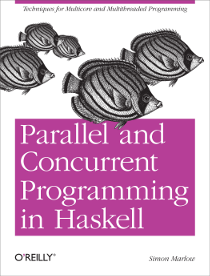
\includegraphics[scale=0.5]{../Woche6/parcur.png} 
\end{center}
\pause

\dots srsly!

\end{frame}

%----------------------------------------------------------------------------------------

\begin{frame}

\begin{center}
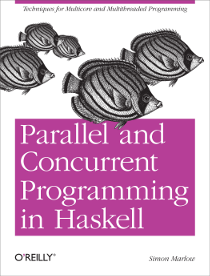
\includegraphics[scale=1]{../Woche6/parcur.png} 
\end{center}

\end{frame}

%----------------------------------------------------------------------------------------

\begin{frame}

\textbf{Überblick:}
\pause

Was war nochmal der Unterschied zwischen Paralllelism und Nebenläufigkeit?

\begin{multicols}{2}
\textbf{Parallelism:}
\begin{itemize}
\item Mehrere Hardwareelemente\pause
\item Antwort schneller kriegen\pause
\item deterministisch (i.d.R.)\pause
\item oft deklarativ\pause
\end{itemize}
\columnbreak
\textbf{Concurrency:}
\begin{itemize}
\item Mehrere Threads\pause
\item Dinge gleichzeitig tun\pause
\item nichtdeterministisch\pause
\item oft impertativ
\end{itemize}
\end{multicols}

\end{frame}

%----------------------------------------------------------------------------------------

\section{Threads, MVars, etc.}

\begin{frame}

\begin{center}
\Large
\textbf{Die Basics: Threads, MVars, etc.}
\end{center}

\end{frame}

%----------------------------------------------------------------------------------------

\subsection{forkIO und MVars}

\begin{frame}[fragile]

Wir beginnen mit der Funktion, die einen neuen Thread erstellt:

\mint{haskell}|forkIO :: IO () -> IO ThreadId|
\pause

Threads interagieren notwendigerweise mit der Welt, ergo ist die Berechnung, die wir 
übergeben vom Typ \texttt{IO ()}.\smallskip\smallskip
\pause

Die \texttt{ThreadId} kann später benutzt werden um z.B. den Thread vorzeitig zu töten oder ihm
eine Exception zuzuschmeißen.
\end{frame}

%----------------------------------------------------------------------------------------

\begin{frame}[fragile]

Ein kleines Beispiel:

\begin{minted}{haskell}
import Control.Concurrent
import Control.Monad
import System.IO

main :: IO ()
main = do
  hSetBuffering stdout NoBuffering
  forkIO (replicateM_ 100000 (putChar 'A')) 
  replicateM_ 100000 (putChar 'B')
\end{minted}
\pause
\dots Output?
\pause
\begin{verbatim}
AAAAAAAAABABABABABABABABABABABABABABABABABABABABABABAB
ABABABABABABABABABABABABABABABABABABABABABABABABABABAB
ABABABABABABABABABABABABABABABABABABABABABABABABABABAB
ABABABABABABABABABABABABABABABABABABABABABABABABABABAB
\end{verbatim}
\end{frame}

%----------------------------------------------------------------------------------------

\begin{frame}[fragile]

Aber\dots \pause wie kriegen wir jetzt Ergebnisse aus der Berechnung raus?\\
Der Typ ist nur \texttt{IO ()}, das liefert nichts (interessantes) zurück!\pause\bigskip

Das gleiche Problem hatten wir schon in der \texttt{Par}-Monade. Lösung damals waren
\texttt{IVar}s:\bigskip

\begin{minted}{haskell}
data IVar a  -- instance Eq

new :: Par (IVar a)
put :: NFData a => IVar a -> a -> Par ()
get :: IVar a -> Par a
\end{minted}
\end{frame}

%----------------------------------------------------------------------------------------

\begin{frame}[fragile]

Introducing: \dots \pause \texttt{MVar}s!\bigskip

\begin{minted}{haskell}
data MVar a  -- abstract

newEmptyMVar :: IO (MVar a)
newMVar      :: a -> IO (MVar a)
takeMVar     :: MVar a -> IO a
putMVar      :: MVar a -> a -> IO ()

readMVar     :: MVar a -> IO a
\end{minted}
\pause

Wir brauchen hier keine eigene Monade wie \texttt{Par}. Da Concurrency so oder so
effektvoll ist, reicht \texttt{IO} vollkommen aus.\bigskip

Unterschied zwischen \texttt{IVar}s und \texttt{MVar}s: erstere sind \emph{\textbf{i}}mmutable,
letztere sind \emph{\textbf{m}}utable.

\end{frame}

%----------------------------------------------------------------------------------------

\begin{frame}[fragile]

Ein Beispiel zu \texttt{MVar}s:

\begin{minted}{haskell}
main :: IO ()
main = do
  m <- newEmptyMVar
  forkIO $ do putMVar m 'x'; putMVar m 'y'
  r <- takeMVar m
  print r
  r <- takeMVar m
  print r
\end{minted}
%$
\pause

Wie wir sehen kann die gleiche \texttt{MVar} über Zeit mehrere Zustände annehmen
und erfolgreich zur Kommunikation zwischen Threads benutzt werden. 

\end{frame}

%----------------------------------------------------------------------------------------

\begin{frame}
Generell haben \texttt{MVar}s drei Hauptaufgaben:\pause

\begin{itemize}
\item \textbf{Channel mit nur einem Slot}\\
Eine \texttt{MVar} kann als Nachrichtenkanal zwischen Threads benutzt werden, allerdings maximal eine Nachricht auf einmal halten.\pause

\item \textbf{Behältnis für shared mutable state}\\
In Concurrent Haskell brauchen oft mehrere Threads Zugriff auf einen shared state. Ein beliebtes Designpattern ist, das dieser State als normaler (immutable) Haskell-Datentyp repräsentiert und in einer \texttt{MVar} verpackt wird.\pause

\item \textbf{Baustein für kompliziertere Strukturen}
\end{itemize}
\end{frame}

%----------------------------------------------------------------------------------------

\subsection{Deadlock Detection}

\begin{frame}[fragile]

\textbf{Mehr Leckerlis:}\smallskip\smallskip

Was passiert, wenn wir folgenden Code ausführen?

\begin{minted}{haskell}
main :: IO ()
main = do m <- newEmptyMVar
          takeMVar m
\end{minted}
\pause
\bigskip

Wir bekommen eine Fehlermeldung, dass das Programm hängt, statt einfach nur ein hängendes Programm.

\begin{verbatim}
$ ./mvar3
mvar3: thread blocked indefinitely in an MVar operation
\end{verbatim}
\end{frame}

%----------------------------------------------------------------------------------------

\begin{frame}
\textbf{Deadlock detection:}

\begin{multicols}{2}
Threads und \texttt{MVar}s sind Objekte auf dem Heap. Das \texttt{RTS} (i.e. der Garbage collector) durchläuft den Heap um alle lebendigen Objekte zu finden, angefangen bei den laufenden Threads und ihren Stacks.\smallskip

Alles was so nicht erreichbar sind (z.B. ein Thread der auf eine \texttt{MVar} wartet, die nirgendwo sonst referenziert wird), blockiert und bekommt eine Exception geschmissen.

\columnbreak

\begin{figure}

\includegraphics[scale=0.52]{dining_philosophers.png} 
\caption{dining philosophers}
\end{figure}

\end{multicols}
\end{frame}

%----------------------------------------------------------------------------------------

\begin{frame}[fragile]

\textbf{Deadlock detection:}\smallskip\smallskip

Dieses Vorgang funktioniert allerdings nicht immer wie man zunächst denkt.
Beispiel: Was passiert mit diesem Code?

\begin{minted}{haskell}
main :: IO ()
main = do 
  lock <- newEmptyMVar
  complete <- newEmptyMVar
  forkIO $ takeMVar lock `finally` putMVar complete ()
  takeMVar complete
\end{minted}
%$
\pause
\bigskip

Da nicht nur der geforkte Thread sondern auch der ursprüngliche gedeadlocked sind, wird hier die Fehlermeldung geprintet, statt die rettende Exception an das Kind zu senden.

\end{frame}

%----------------------------------------------------------------------------------------

\section{Software Transactional Memory}

\begin{frame}

\begin{center}
\Large
\textbf{Software Transactional Memory (STM)}
\end{center}


\end{frame}

%----------------------------------------------------------------------------------------

\subsection{Motivation}

\begin{frame}

\textbf{Motivation:}\smallskip

Trotz aller Unterstützung durch das \texttt{RTS}:\pause

\begin{center}
\emph{Locks are absurdly hard to get right!} (SPJ)
\end{center}
\tiny \glqq The Future is Parallel, and the Future of Parallel is Declarative \grqq
\vspace{-5pt} \\
 https://www.youtube.com/watch?v=hlyQjK1qjw8\normalsize
\pause
\smallskip\smallskip

Beliebte Fehler:

\begin{itemize}
\item \textbf{Races} (vergessene Locks)\pause
\item \textbf{Deadlocks} (Locks in falscher Reihenfolge genommen)\pause
\item \textbf{Lost wakeups} (Conditional-Variable nicht bescheid gesagt)\pause
\item \textbf{Error Recovery} (Exceptionhandler müssen Locks freigeben und teilweise Ursprungszustand restaurieren)
\end{itemize}

\end{frame}

%----------------------------------------------------------------------------------------

\begin{frame}

\textbf{Beispiel:}\bigskip

Angenommen wir möchten gerne eine Queue parallel bearbeiten:\\
\tiny Bildquelle: http://www.math.bas.bg/$\sim$nkirov/2015/NETB201/slides/ch04/ch04.html \normalsize

\begin{center}
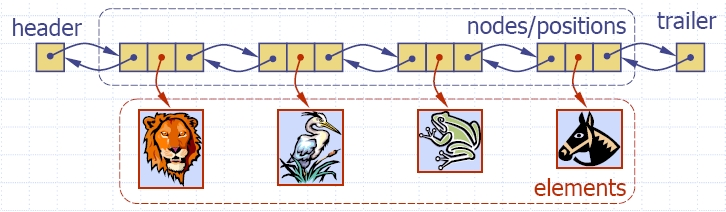
\includegraphics[scale=0.35]{liste_frei.jpg} 
\end{center}
\pause

Problem: offensichtlich, race conditions etc.

\end{frame}

%----------------------------------------------------------------------------------------

\begin{frame}

\textbf{Beispiel:}\bigskip

Angenommen wir möchten gerne eine Queue parallel bearbeiten:\\
\tiny Bildquelle: http://www.math.bas.bg/$\sim$nkirov/2015/NETB201/slides/ch04/ch04.html \normalsize

\begin{center}
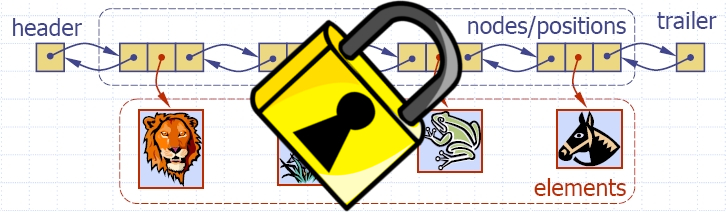
\includegraphics[scale=0.35]{liste_locked.jpg} 
\end{center}
\pause

Problem: Nicht gerade nebenläufig\dots

\end{frame}

%----------------------------------------------------------------------------------------

\begin{frame}

\textbf{Beispiel:}\bigskip

Angenommen wir möchten gerne eine Queue parallel bearbeiten:\\
\tiny Bildquelle: http://www.math.bas.bg/$\sim$nkirov/2015/NETB201/slides/ch04/ch04.html \normalsize

\begin{center}
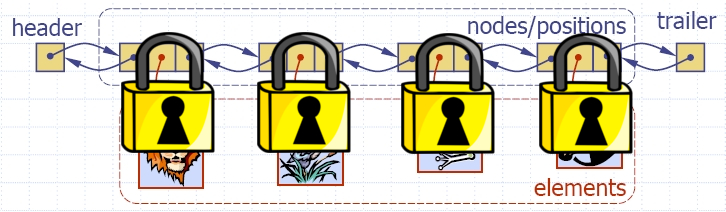
\includegraphics[scale=0.35]{liste_individually_locked.jpg} 
\end{center}
\pause

Problem: Fehleranfälligkeit bei kleinen Listen

\end{frame}

%----------------------------------------------------------------------------------------

\begin{frame}

Aufgabe vs. Schwierigkeit: Zweiendige Liste\bigskip

\begin{center}
\begin{tabular}{c|c}
Problemstellung & Schwierigkeit \\
\hline \\
sequentiell & Gymnasium oder Bachelor \pause \\ \\
Locks et al. & (gerade nicht mehr) publizierbar \\ & auf internationalen Konferenzen \pause \\ \\
atomic blocks (\texttt{STM}) & Bachelor
\end{tabular}
\end{center}

\end{frame}

%----------------------------------------------------------------------------------------

\begin{frame}[fragile]

Software Transactional Memory stellt die Möglichkeit zur Verfügung, Berechnungen in atomaren (d.h. nicht unterbrochenen) Blöcken auszuführen. Das Interface ist aber das gleiche, wie in wie jeder anderen Monade auch (\texttt{do}-Notation etc.).\pause\bigskip

\begin{itemize}
\item Das bedeutet, dass Deadlocks unmöglich werden \emph{weil es keine Locks mehr gibt}!\pause
\item Automatisierte error recovery. \texttt{STM} stellt den Ausgangszustand von selbst wieder her.\pause
\item \texttt{TVar}s (Transaction Variables). Wie \texttt{IVar}s und \texttt{MVar}s, nur in der \texttt{STM}-Monade.
\end{itemize}

\end{frame}

%----------------------------------------------------------------------------------------

\begin{frame}[fragile]

\underline{\texttt{STM} auf einen Blick:}\bigskip

\begin{minted}{haskell}
data STM a                        -- abstract
instance Monad STM                -- among other things

atomically :: STM a -> IO a

data TVar a                       -- abstract
newTVar   :: a -> STM (TVar a)
readTVar  :: TVar a -> STM a
writeTVar :: TVar a -> a -> STM ()

retry     :: STM a
orElse    :: STM a -> STM a -> STM a

throwSTM  :: Exception e => e -> STM a
catchSTM  :: Exception e => STM a -> (e -> STM a) -> STM a
\end{minted}

\end{frame}

%----------------------------------------------------------------------------------------

\begin{frame}[fragile]

Ein kurzer Blick auf \texttt{atomically}:

\mint{haskell}|atomically :: STM a -> IO a|
\pause

\begin{itemize}
\item \emph{Kein} Sprachkonstrukt!\pause
\item Führt Berechnungen in \texttt{STM} in der echten Welt aus\pause
\item \dots und zwar in einem Rutsch, ohne Unterbrechung!\pause
\item Stellt bei Fehlschlag Ursprungszustand wieder her.\pause
\item Deshalb: Kein \texttt{IO} in Transaktionen!\pause
\item Ebenfalls: Keine genesteten \texttt{atomically}s (Typen!) 
\end{itemize}
\end{frame}

%----------------------------------------------------------------------------------------

\begin{frame}[fragile]

Ein kurzer Blick auf \texttt{retry}:

\mint{haskell}|retry :: STM a|
\pause

\begin{itemize}
\item \emph{Kein} Sprachkonstrukt!\pause
\item Rollt zurück und versucht die gleiche Transaktion erneut durchzuführen\pause
\item \dots allerdings erst zu einem angebrachten Zeitpunkt.\\ CPU wird nicht unnützerweise zur Heizung.\pause
\end{itemize}
\end{frame}

%----------------------------------------------------------------------------------------

\begin{frame}[fragile]

Ein kurzer Blick auf \texttt{orElse}:

\mint{haskell}|orElse :: STM a -> STM a -> STM a|
\pause

\begin{itemize}
\item \emph{Kein} Sprachkonstrukt!\pause
\item \texttt{orElse a b} führt \texttt{b} aus, wenn \texttt{a} \texttt{retry} aufruft.\pause
\item Komposition von \texttt{STM}-Berechnungen:\\
\texttt{>>=} ist \texttt{AND}; \texttt{orElse} ist \texttt{OR}
\end{itemize}
\pause

Beispiel:
\begin{minted}{haskell}
takeEitherTMVar :: TMVar a -> TMVar b -> STM (Either a b)
takeEitherTMVar ma mb =
  fmap Left (takeTMVar ma)
    `orElse`
  fmap Right (takeTMVar mb)
\end{minted}
\end{frame}

%----------------------------------------------------------------------------------------

\subsection{Beispiel: Banksoftware}

\begin{frame}[fragile]

Stellen wir uns vor, wir wollen eine simplifizierte Bankensoftware schreiben, die in der Lage sein soll, Konten und Überweisungen zu repräsentieren.\pause\bigskip

Eine naive Implementation wäre die folgende:

\begin{minted}{haskell}
type Account = IORef Integer
 
transfer :: Integer -> Account -> Account -> IO ()
transfer amount from to = do
    fromVal <- readIORef from
    toVal   <- readIORef to
    writeIORef from (fromVal - amount)
    writeIORef to (toVal + amount)
\end{minted}
\end{frame}

%----------------------------------------------------------------------------------------

\begin{frame}[fragile]

Diese Implementation hätte jedoch in einem Nebenläufigen Setting einige Probleme. Man beachte folgende Zeile:

\begin{minted}{haskell}
fromVal <- readIORef from
\end{minted}
\pause

Finden nun mehrere Aktionen gleichzeitig statt, so könnte es sein, dass mehrere Threads denselben Wert als \texttt{fromVal} lesen, bevor die jeweils andere Transaktion durchgeführt wurde.

Dies hätte zur Folge, dass später ein inkorrekter Kontostand berechnet und gesetzt würde.

\end{frame}

%----------------------------------------------------------------------------------------

\begin{frame}[fragile]

Führen wir also Locks ein (durch Benutzung von \texttt{MVar}s), um diese race condition zu verhindern. \pause\smallskip

\begin{minted}{haskell}
type Account = MVar Integer
 
credit :: Integer -> Account -> IO ()
credit amount account = do
    current <- takeMVar account
    putMVar account (current + amount)
 
debit :: Integer -> Account -> IO ()
debit amount account = do
    current <- takeMVar account
    putMVar account (current - amount)

\end{minted}

\end{frame}

%----------------------------------------------------------------------------------------

\begin{frame}[fragile]

In dieser Implementation sähe eine Funktion für Überweisungen etwa so aus:

\begin{minted}{haskell}
transfer :: Integer -> Account -> Account -> IO ()
transfer amount from to = do
    debit  amount from
    credit amount to
\end{minted}
\pause

Diese verhindert, dass durch fehlerhaftes Zusammenspiel von Threads Geld geschaffen oder
vernichtet wird.\pause\smallskip\smallskip

Es existiert allerdings immer noch eine race condition: Der Thread, der die Überweisung ausführt, könnte direkt nach dem \texttt{debit}-Schritt von der CPU verdrängt werden und die Bankensoftware dadurch in einem inkonsistenten Zustand zurück lassen.

\end{frame}

%----------------------------------------------------------------------------------------

\begin{frame}[fragile]

Wie sähe diese Software mit \texttt{STM} aus?

\begin{minted}{haskell}
type Account = TVar Integer
 
credit :: Integer -> Account -> STM ()
credit amount account = do
    current <- readTVar account
    writeTVar account (current + amount)
 
debit :: Integer -> Account -> STM ()
debit amount account = do
    current <- readTVar account
    writeTVar account (current - amount)
 
transfer :: Integer -> Account -> Account -> STM ()
transfer amount from to = do
    debit  amount from
    credit amount to
\end{minted}
\end{frame}

%----------------------------------------------------------------------------------------

\begin{frame}[fragile]

Vergleich zur Variante mit \texttt{MVar}s:

\begin{minted}{haskell}
type Account = MVar Integer
 
credit :: Integer -> Account -> IO ()
credit amount account = do
    current <- takeMVar account
    putMVar account (current + amount)
 
debit :: Integer -> Account -> IO ()
debit amount account = do
    current <- takeMVar account
    putMVar account (current - amount)
 
transfer :: Integer -> Account -> Account -> IO ()
transfer amount from to = do
    debit  amount from
    credit amount to
\end{minted}
\end{frame}

%----------------------------------------------------------------------------------------

\begin{frame}[fragile]

Der Unterschied hier besteht hauptsächlich in den Rückgabetypen.\pause

\mint{haskell}|transfer :: Integer -> Account -> Account -> IO ()|

Diese Funktion führt die Überweisung vollkommen in der echten Welt durch, mit allen
möglichen Fehlern, die dabei auftreten können.\pause

\mint{haskell}|transfer :: Integer -> Account -> Account -> STM ()|

Diese Funktion stellt uns nur eine Berechnung in der \texttt{STM}-Monade bereit, die wir
später entweder direkt oder auch als Baustein einer größeren Transaktion ausführen können.\pause

Der Vorteil ist, dass wir nur einen Weg haben, diese Berechnung haben, das zu tun:
\mint{haskell}|atomically :: STM a -> IO a|
\end{frame}

%----------------------------------------------------------------------------------------

\begin{frame}
Wenn wir doch jetzt dieses tolle \texttt{STM} haben, brauchen wir dann überhaupt noch \texttt{MVar}s?\pause\bigskip

Ja! Hier sind einige Gründe:\pause
\begin{itemize}
\item \textbf{Performance:} \texttt{STM} ist eine Abstraktion, und wie (fast) alle Abstraktionen hat es Laufzeitkosten.\pause
\item \textbf{Fairness:} Blockieren mehrere Threads auf einer \texttt{MVar}, werden sie garantiert FIFO wieder aufgeweckt. \texttt{STM} hingegen hat keine Garantie für Fairness.
\end{itemize} 
\end{frame}

%----------------------------------------------------------------------------------------

\section{Ein simpler Chat-Server}

\begin{frame}

\begin{center}
\Large
\textbf{Hands on:\\Ein einfacher Chat-Server in Haskell}
\end{center}

\end{frame}

%----------------------------------------------------------------------------------------

\begin{frame}

Wir wollen uns einen simplen Chat-Server basteln, der Verbindungen mit mehreren Clients 
(verbunden über \texttt{telnet}) gleichzeitig offen halten und bearbeiten kann.\pause\bigskip

Insbesondere sollen einem Client folgende Befehle offen stehen:
\begin{enumerate}
\item \emph{/tell name} Schickt eine private Nachricht an den User \emph{name}\pause
\item \emph{/kick name} Disconnectet den User \emph{name}\pause
\item \emph{/quit} Disconnected den aktuellen Client selbst\pause
\item \emph{message} Alle anderen Strings werden an alle verbundenen Clients gebroadcastet.
\end{enumerate}

\end{frame}

%----------------------------------------------------------------------------------------

\begin{frame}[fragile]

Ein sinnvoller erster Schritt ist oft, zu überlegen, wie man seine grundlegenden Datentypen
repräsentieren möchte.\smallskip\smallskip

Bei uns sind das inbesondere Clients und Nachrichten:\pause\smallskip\smallskip

\begin{minted}{haskell}
type ClientName = String -- zum besseren Verständnis

data Client = Client
  { clientName     :: ClientName
  , clientHandle   :: Handle
  , clientKicked   :: TVar (Maybe String)
  , clientSendChan :: TChan Message
  }
\end{minted}
\pause
\texttt{TChan}s sind FIFO Channel zur Kommunikation zwischen Threads, ebenfalls ein \texttt{STM} primitive.
\end{frame}

%----------------------------------------------------------------------------------------

\begin{frame}[fragile] 

Nachrichten sind ebenfalls schnell implementiert:\pause

\begin{minted}{haskell}
data Message = Notice String
             | Tell ClientName String
             | Broadcast ClientName String
             | Command String
\end{minted}

Wobei \texttt{Notice} eine Nachricht vom Server, \texttt{Tell} eine private Nachricht, \texttt{Broadcast} eine
öffentliche Nachricht und \texttt{Command} ein Befehl vom Nutzer ist.
\end{frame}

%----------------------------------------------------------------------------------------

\begin{frame}[fragile]

Neue Clients zu erstellen ist für's Erste ziemlich einfach (vorausgesetzt \texttt{Handle} und 
\texttt{ClientName} werden übergeben):\smallskip

\begin{minted}{haskell}
newClient :: ClientName -> Handle -> STM Client
newClient name handle = do
  c <- newTChan
  k <- newTVar Nothing
  return Client { clientName     = name
                , clientHandle   = handle
                , clientSendChan = c
                , clientKicked   = k
                }
\end{minted}
\pause
Man beachte, dass der Rückgabewert ein \texttt{Client} in \texttt{STM} ist!
\pause
      
\begin{minted}{haskell}          
sendMessage :: Client -> Message -> STM ()
sendMessage Client{..} msg =
  writeTChan clientSendChan msg
\end{minted}

Die \texttt{\{..\}}-Syntax nennt sich \emph{record wildcard}-Syntax (benötigt die Extension \texttt{RecordWildCards}). Diese holt alle Felder des Records mit ihren respektiven Namen in scope.

\end{frame}

%----------------------------------------------------------------------------------------

\begin{frame}[fragile]

Ein Server ist in unserem Falle eine Key-Value-Map von \texttt{ClientName}s zu \texttt{Client}s. Das bedeutet jedem Namen wird genau ein Client zugeordnet.

(importiert aus \texttt{Data.Map}, nicht zu verwechseln mit \texttt{map} für Listen)\smallskip

Diese Map wird in einer \texttt{TVar} vorgehalten.\bigskip

\begin{minted}{haskell}
data Server = Server
  { clients :: TVar (Map ClientName Client)
  }
\end{minted}

\end{frame}
  
  
%----------------------------------------------------------------------------------------

\begin{frame}[fragile] 

Eine Funktion für neue Server ist schnell erstellt. Hier ist es nicht notwendig, in 
\texttt{STM} zu bleiben.

\begin{minted}{haskell}
newServer :: IO Server
newServer = do
  c <- newTVarIO Map.empty
  return Server { clients = c }
\end{minted}
\end{frame}

%----------------------------------------------------------------------------------------

\begin{frame}[fragile]
Wollen wir nun also eine Nachricht über einen ganzen \texttt{Server} verschicken, 
(Broadcast), nehmen wir uns einfach alle Elemente der Map einzeln.

\begin{minted}{haskell}
broadcast :: Server -> Message -> STM ()
broadcast Server{..} msg = do
  clientmap <- readTVar clients
  mapM_ (\client -> sendMessage client msg)
                           (Map.elems clientmap)
\end{minted}
\pause

\texttt{mapM\_} ist das \texttt{map} auf Listen, nur dass das (monadische) Ergebnis jeweils weggeschmissen wird.
\smallskip

\mint{haskell}|mapM_ :: (Monad m, Foldable t) => (a -> m b) -> t a -> m ()|
\end{frame}

%----------------------------------------------------------------------------------------

\begin{frame}[fragile]

Wir brauchen einen Port, auf dem der Server lauschen soll. Eigentlich egal welcher, solange wir nicht einen beliebten Standardport nehmen. 

\begin{minted}{haskell}
port :: Int
port = 44444
\end{minted}
\end{frame}

%----------------------------------------------------------------------------------------

\begin{frame}[fragile]

\begin{minted}{haskell}
main :: IO ()
main = withSocketsDo $ do
  server <- newServer
  sock <- listenOn (PortNumber (fromIntegral port))
  printf "Listening on port %d\n" port
  forever $ do
    (handle, host, port) <- accept sock
    printf "Accepted connection from %s: %s\n" host (show port)
    forkFinally (talk handle server) (\_ -> hClose handle)
\end{minted}
\pause

\texttt{accept} blockiert bis eine neue Verbindung hergestellt wurde.\pause\smallskip\smallskip

Mit \texttt{forkFinally} erstellen wir einen neuen Thread um die Interaktion mit diesem Client
(über die noch zu schreibende Funktion \texttt{talk}) zu regeln und sobald das beendet ist den Handle
sinnvoll zu beenden.

\end{frame}

%----------------------------------------------------------------------------------------

\begin{frame}[fragile]

Clients werden atomar hionzugefügt, damit sich nicht zwei Clients gleichzeitig
mit demselben Namen anmelden können.

\begin{minted}{haskell}
checkAddClient :: Server -> ClientName -> Handle
                                       -> IO (Maybe Client)
checkAddClient server@Server{..} name handle = atomically $ do
  clientmap <- readTVar clients
  if Map.member name clientmap
    then return Nothing
    else do 
       client <- newClient name handle
       writeTVar clients $ Map.insert name client clientmap
       broadcast server  $ Notice (name ++ " has connected")
       return (Just client)
\end{minted}
%$
\end{frame}

%----------------------------------------------------------------------------------------

\begin{frame}[fragile]

Clients entfernen funktioniert ähnlich, ebenfalls atomar:

\begin{minted}{haskell}
removeClient :: Server -> ClientName -> IO ()
removeClient server@Server{..} name = atomically $ do
  modifyTVar' clients $ Map.delete name
  broadcast server $ Notice (name ++ " has disconnected")
\end{minted}
%$
\end{frame}

%----------------------------------------------------------------------------------------

\begin{frame}[fragile]

\begin{minted}{haskell}
talk :: Handle -> Server -> IO ()
talk handle server@Server{..} = do
  hSetNewlineMode handle universalNewlineMode
      -- Swallow carriage returns sent by telnet clients
  hSetBuffering handle LineBuffering
  readName
 where
  readName = do
    hPutStrLn handle "What is your name?"
    name <- hGetLine handle
    if null name
      then readName
      else mask $ \restore -> do
             ok <- checkAddClient server name handle
             case ok of
               Nothing -> restore $ do
                  hPrintf handle
                     "The name %s is already in use.\n" name
                  readName
               Just client ->
                  restore (runClient server client)
                      `finally` removeClient server name
\end{minted}

\end{frame}

%----------------------------------------------------------------------------------------

\begin{frame}[fragile]

\begin{minted}{haskell}
runClient :: Server -> Client -> IO ()
runClient serv@Server{..} client@Client{..} = do
  race server receive
  return ()
 where
  receive = forever $ do
    msg <- hGetLine clientHandle
    atomically $ sendMessage client (Command msg)

  server = join $ atomically $ do
    k <- readTVar clientKicked
    case k of
      Just reason -> return $
        hPutStrLn clientHandle $
              "You have been kicked: " ++ reason
      Nothing -> do
        msg <- readTChan clientSendChan
        return $ do
            continue <- handleMessage serv client msg
            when continue $ server
\end{minted}

\end{frame}

%----------------------------------------------------------------------------------------

\begin{frame}[fragile]

\begin{minted}[fontsize=\tiny]{haskell}
handleMessage :: Server -> Client -> Message -> IO Bool
handleMessage server client@Client{..} message =
  case message of
     Notice msg         -> output $ "*** " ++ msg
     Tell name msg      -> output $ "*" ++ name ++ "*: " ++ msg
     Broadcast name msg -> output $ "<" ++ name ++ ">: " ++ msg
     Command msg ->
       case words msg of
           ["/kick", who] -> do
               atomically $ kick server who clientName
               return True
           "/tell" : who : what -> do
               tell server client who (unwords what)
               return True
           ["/quit"] ->
               return False
           ('/':_):_ -> do
               hPutStrLn clientHandle $ "Unrecognized command: " ++ msg
               return True
           _ -> do
               atomically $ broadcast server $ Broadcast clientName msg
               return True
 where
   output s = do hPutStrLn clientHandle s; return True
\end{minted}
%$

\end{frame}

\end{document}
